% %%%%%%%%%%%%%%%%%%%%%%%%%%%%%%%%%%%%%%%%%%%%%%%%%%%%%%%%%%%%%%%%%%%
% moe_architecture.tex
% Board-type mixture-of-experts reconstruction model (target design).
%
% Compiles with:  pdflatex moe_architecture.tex
% Size: designed for a full-width (17 cm) figure in a two-column paper.
%
% Ground truth:
%   expert network   tdp/unet/model.py   (base 24, depth 3, 538,753 params)
%   input contract   tdp/unet/train.py   (3 channels; L1 over board pixels)
%   routing          tmp/experimental_principles_draft.md eq. (3.4)-(3.5)
%   board grids      configs/measurements_v3.yaml (157 x 103),
%                    configs/measurements_opi5pro.yaml (164 x 103)
%
% Suggested caption (outside the artwork):
%   Board-type mixture-of-experts reconstruction of the infrared
%   temperature field. (a) Every board type owns one residual U-Net
%   expert with identical topology but separate weights, operating on
%   that board's own grid (157 x 103 for the Raspberry Pi 4B, 164 x 103
%   for the Orange Pi 5 Pro); a deterministic router reads the board
%   type from the session record and enables exactly one expert per
%   sample as a one-hot lookup, with no gating weights and no averaging
%   of expert outputs. The selected expert outputs a temperature
%   correction in kelvin, which is added to the input temperature field.
%   (b) One expert in detail: a three-level residual U-Net (24/48/96
%   channels, group norm, SiLU) trained with complete-map L1 over board
%   pixels. The routing layer is a target design; the experiments
%   reported in this work use a single expert (K = 1).
% %%%%%%%%%%%%%%%%%%%%%%%%%%%%%%%%%%%%%%%%%%%%%%%%%%%%%%%%%%%%%%%%%%%
\documentclass[border=3pt]{standalone}
\usepackage[T1]{fontenc}
\usepackage[scaled=0.92]{helvet}
\renewcommand{\familydefault}{\sfdefault}
\usepackage{tikz}
\usetikzlibrary{arrows.meta, patterns}

\definecolor{active}{HTML}{0072B2}   % Okabe-Ito blue: active routing path
\definecolor{resid}{HTML}{D55E00}    % Okabe-Ito vermillion: residual path
\definecolor{inactive}{HTML}{9A9A9A} % grey: paths not evaluated
\definecolor{ink}{HTML}{1F1F1F}

\tikzset{
  arr/.style={draw=ink, line width=0.6pt, -{Stealth[length=1.8mm]}},
  arrthin/.style={draw=ink, line width=0.5pt, -{Stealth[length=1.5mm]}},
  boxlabel/.style={font=\sffamily\scriptsize, align=center, inner sep=1.5pt},
  ann/.style={font=\sffamily\fontsize{6.3}{7.0}\selectfont, align=center, inner sep=1pt},
  annpar/.style={font=\sffamily\fontsize{6.3}{7.2}\selectfont, align=justify,
                 inner sep=0pt},
  pbox/.style={draw=ink, line width=0.5pt, boxlabel, minimum width=1.4cm,
               inner sep=2.5pt},
}

\begin{document}
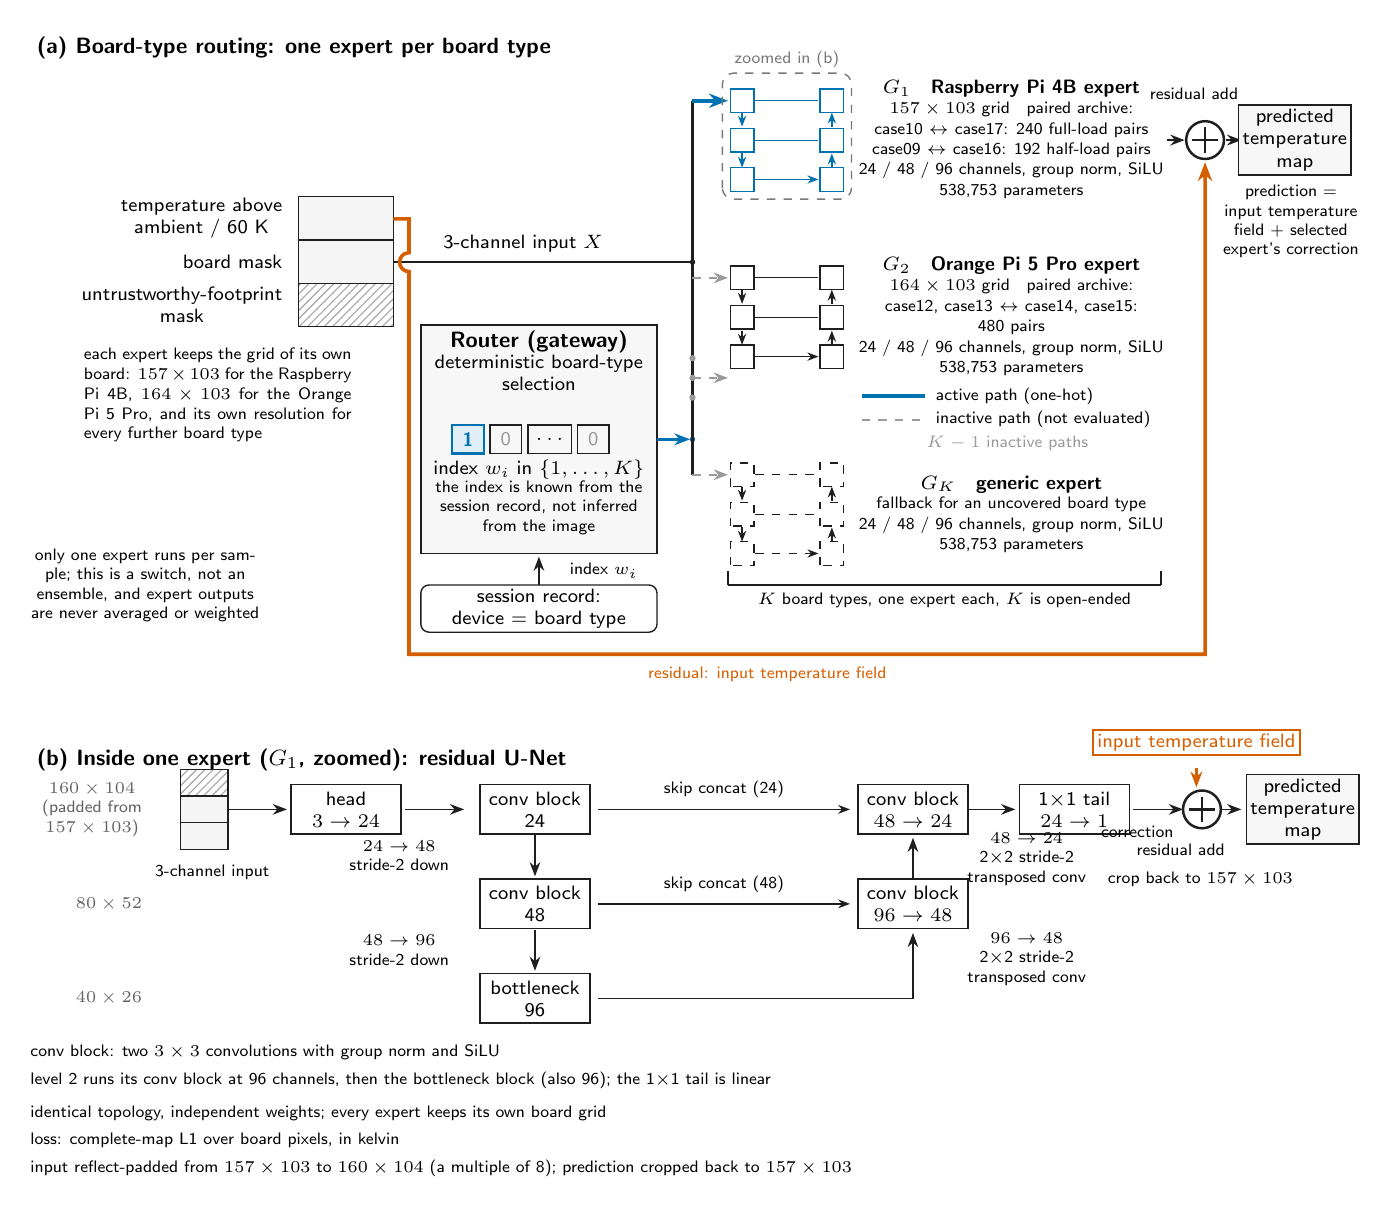
\begin{tikzpicture}[x=1cm, y=1cm]

% =================== PANEL (a): routing level =====================
\node[font=\sffamily\footnotesize\bfseries, anchor=west] at (0,7.72)
  {(a) Board-type routing: one expert per board type};

% ---- input stack (three channel maps) -----------------------------
\draw[ink, line width=0.5pt, fill=black!4]
  (3.45,5.28) rectangle (4.65,5.83);
\draw[ink, line width=0.5pt, fill=black!4]
  (3.45,4.73) rectangle (4.65,5.28);
\draw[ink, line width=0.5pt, pattern=north east lines, pattern color=black!35]
  (3.45,4.18) rectangle (4.65,4.73);
\node[boxlabel, anchor=east] at (3.30,5.555)
  {temperature above\\ambient / 60 K};
\node[boxlabel, anchor=east] at (3.30,5.005) {board mask};
\node[boxlabel, anchor=east] at (3.30,4.455)
  {untrustworthy-footprint\\mask};

% per-board grid annotation under the stack
\node[annpar, text width=3.4cm, anchor=north] at (2.42,3.92)
  {each expert keeps the grid of its own board:
   $157\times103$ for the Raspberry Pi~4B, $164\times103$ for the
   Orange Pi~5 Pro, and its own resolution for every further board type};

% ---- X bus: 3-channel input to the expert columns ------------------
\draw[ink, line width=0.9pt] (4.65,5.0) -- (8.45,5.0);
\node[boxlabel] at (6.3,5.24) {3-channel input $X$};
\fill[ink] (8.45,5.0) circle (0.035);

% ---- router / gateway ----------------------------------------------
\draw[ink, line width=0.6pt, fill=black!3] (5.0,1.30) rectangle (8.0,4.20);
\node[font=\sffamily\footnotesize\bfseries] at (6.5,3.98) {Router (gateway)};
\node[boxlabel] at (6.5,3.60) {deterministic board-type\\selection};
% one-hot vector cells [1 0 ... 0]
\draw[active, line width=0.8pt, fill=active!12] (5.40,2.57) rectangle (5.80,2.93);
\node[font=\sffamily\scriptsize\bfseries, text=active] at (5.60,2.75) {1};
\draw[ink, line width=0.5pt] (5.88,2.57) rectangle (6.28,2.93);
\node[boxlabel, text=inactive] at (6.08,2.75) {0};
\draw[ink, line width=0.5pt] (6.36,2.57) rectangle (6.91,2.93);
\node[boxlabel] at (6.635,2.75) {$\ldots$};
\draw[ink, line width=0.5pt] (6.99,2.57) rectangle (7.39,2.93);
\node[boxlabel, text=inactive] at (7.19,2.75) {0};
\node[boxlabel] at (6.5,2.36) {index $w_i$ in $\{1,\ldots,K\}$};
\node[ann] at (6.5,1.88)
  {the index is known from the\\session record, not inferred\\from the image};

% session-record metadata tag (routing key), feeding the router from below
\draw[ink, line width=0.5pt, rounded corners=3pt, fill=white]
  (5.0,0.30) rectangle (8.0,0.90);
\node[boxlabel] at (6.5,0.60) {session record:\\device = board type};
\draw[arr] (6.5,0.90) -- (6.5,1.26);
\node[ann, anchor=west] at (6.85,1.08) {index $w_i$};

% router -> dispatch bus (the one-hot selection)
\draw[active, line width=1.2pt, -{Stealth[length=2mm]}] (8.0,2.75) -- (8.42,2.75);
\fill[active] (8.45,2.75) circle (0.035);

% ---- dispatch bus + branches ---------------------------------------
\draw[ink, line width=0.9pt] (8.45,2.3) -- (8.45,7.05);
\draw[active, line width=1.6pt, -{Stealth[length=2.4mm]}] (8.45,7.05) -- (8.90,7.05);
\draw[inactive, line width=0.8pt, dashed, -{Stealth[length=1.8mm]}]
  (8.45,4.8) -- (8.90,4.8);
\draw[inactive, line width=0.8pt, dashed, -{Stealth[length=1.8mm]}]
  (8.45,3.53) -- (8.90,3.53);
\draw[inactive, line width=0.8pt, dashed, -{Stealth[length=1.8mm]}]
  (8.45,2.30) -- (8.90,2.30);
\foreach \dy in {3.28,3.53,3.78} \fill[inactive] (8.45,\dy) circle (0.04);

% ---- expert glyph ---------------------------------------------------
\newcommand{\expertglyph}[3]{% center x, center y, style
\begin{scope}[shift={(#1,#2)}, #3]
  \foreach \yy in {0.5,0,-0.5} {
    \draw[line width=0.5pt, fill=white] (-0.72,\yy-0.15) rectangle (-0.42,\yy+0.15);
    \draw[line width=0.5pt, fill=white] ( 0.42,\yy-0.15) rectangle ( 0.72,\yy+0.15);}
  \draw[line width=0.5pt, -{Stealth[length=1.4mm]}] (-0.57, 0.35) -- (-0.57, 0.17);
  \draw[line width=0.5pt, -{Stealth[length=1.4mm]}] (-0.57,-0.17) -- (-0.57,-0.35);
  \draw[line width=0.5pt, -{Stealth[length=1.4mm]}] (-0.40,-0.50) -- ( 0.40,-0.50);
  \draw[line width=0.5pt, -{Stealth[length=1.4mm]}] ( 0.57,-0.35) -- ( 0.57,-0.17);
  \draw[line width=0.5pt, -{Stealth[length=1.4mm]}] ( 0.57, 0.17) -- ( 0.57, 0.35);
  \draw[line width=0.4pt] (-0.40, 0.50) -- ( 0.40, 0.50);
  \draw[line width=0.4pt] (-0.40, 0.00) -- ( 0.40, 0.00);
\end{scope}}

% zoom callout around expert 1's glyph
\draw[ink!60, line width=0.5pt, dashed, rounded corners=4pt]
  (8.83,5.80) rectangle (10.47,7.40);
\node[ann, text=ink!60] at (9.65,7.58) {zoomed in (b)};

% ---- expert rows ----------------------------------------------------
% Expert 1 (selected)
\expertglyph{9.65}{6.55}{draw=active, fill=white}
\node[boxlabel] at (12.5,7.20) {\textbf{$G_1$ \; Raspberry Pi 4B expert}};
\node[ann] at (12.5,6.94) {$157\times103$ grid \; paired archive:};
\node[ann] at (12.5,6.68) {case10 $\leftrightarrow$ case17: 240 full-load pairs};
\node[ann] at (12.5,6.42) {case09 $\leftrightarrow$ case16: 192 half-load pairs};
\node[ann] at (12.5,6.16) {24 / 48 / 96 channels, group norm, SiLU};
\node[ann] at (12.5,5.90) {538{,}753 parameters};

% Expert 2
\expertglyph{9.65}{4.30}{draw=ink, fill=white}
\node[boxlabel] at (12.5,4.95) {\textbf{$G_2$ \; Orange Pi 5 Pro expert}};
\node[ann] at (12.5,4.69) {$164\times103$ grid \; paired archive:};
\node[ann] at (12.5,4.43) {case12, case13 $\leftrightarrow$ case14, case15:};
\node[ann] at (12.5,4.17) {480 pairs};
\node[ann] at (12.5,3.91) {24 / 48 / 96 channels, group norm, SiLU};
\node[ann] at (12.5,3.65) {538{,}753 parameters};

% Expert K (generic fallback, dashed)
\expertglyph{9.65}{1.80}{draw=ink, dashed, fill=white}
\node[boxlabel] at (12.5,2.18) {\textbf{$G_K$ \; generic expert}};
\node[ann] at (12.5,1.92) {fallback for an uncovered board type};
\node[ann] at (12.5,1.66) {24 / 48 / 96 channels, group norm, SiLU};
\node[ann] at (12.5,1.40) {538{,}753 parameters};

% ---- legend + count --------------------------------------------------
\draw[active, line width=1.6pt] (10.60,3.30) -- (11.40,3.30);
\node[ann, anchor=west] at (11.50,3.30) {active path (one-hot)};
\draw[inactive, line width=0.8pt, dashed] (10.60,3.00) -- (11.40,3.00);
\node[ann, anchor=west] at (11.50,3.00) {inactive path (not evaluated)};
\node[ann, text=inactive] at (12.45,2.70) {$K-1$ inactive paths};

% ---- group bracket ---------------------------------------------------
\draw[ink, line width=0.5pt] (8.90,0.90) -- (8.90,1.08);
\draw[ink, line width=0.5pt] (14.40,0.90) -- (14.40,1.08);
\draw[ink, line width=0.5pt] (8.90,0.90) -- (14.40,0.90);
\node[ann, anchor=north] at (11.65,0.84)
  {$K$ board types, one expert each, $K$ is open-ended};

% ---- side note (switch, not ensemble) --------------------------------
\node[ann, text width=2.9cm, anchor=north] at (1.5,1.40)
  {only one expert runs per sample; this is a switch, not an
   ensemble, and expert outputs are never averaged or weighted};

% ---- residual add + output -------------------------------------------
\draw[arr, line width=0.9pt] (14.48,6.55) -- (14.70,6.55);
\draw[ink, line width=0.9pt] (14.96,6.55) circle (0.24);
\draw[ink, line width=0.9pt] (14.80,6.55) -- (15.12,6.55);
\draw[ink, line width=0.9pt] (14.96,6.39) -- (14.96,6.71);
\node[ann] at (14.82,7.14) {residual add};
\draw[arr, line width=0.9pt] (15.22,6.55) -- (15.42,6.55);
\node[boxlabel, draw=ink, line width=0.6pt, fill=black!3] at (16.10,6.55)
  {predicted\\temperature\\map};
\node[ann, anchor=north] at (16.05,6.02)
  {prediction =\\input temperature\\field + selected\\expert's correction};

% residual path: input temperature channel, around the bottom, up to the add
\draw[resid, line width=1.3pt]
  (4.65,5.55) -- (4.85,5.55) -- (4.85,5.12)
  arc[start angle=90, end angle=270, radius=0.12]
  -- (4.85,0.02) -- (14.96,0.02) -- (14.96,6.07);
\draw[resid, line width=1.3pt, -{Stealth[length=2.4mm]}] (14.96,6.07) -- (14.96,6.27);
\node[ann, text=resid] at (9.4,-0.24) {residual: input temperature field};

% ================= PANEL (b): inside one expert =====================
\node[font=\sffamily\footnotesize\bfseries, anchor=west] at (0,-1.32)
  {(b) Inside one expert ($G_1$, zoomed): residual U-Net};

% spatial-size gutter (Pi 4B grid, height x width)
\node[ann, text=ink!70, anchor=east] at (1.50,-1.95)
  {$160\times104$\\(padded from\\$157\times103$)};
\node[ann, text=ink!70, anchor=east] at (1.50,-3.15) {$80\times52$};
\node[ann, text=ink!70, anchor=east] at (1.50,-4.35) {$40\times26$};

% input stack
\draw[ink, line width=0.5pt, fill=black!4] (1.95,-1.95-0.51) rectangle (2.55,-1.95-0.17);
\draw[ink, line width=0.5pt, fill=black!4] (1.95,-1.95-0.17) rectangle (2.55,-1.95+0.17);
\draw[ink, line width=0.5pt, pattern=north east lines, pattern color=black!35]
  (1.95,-1.95+0.17) rectangle (2.55,-1.95+0.51);
\node[ann, anchor=north] at (2.35,-2.62) {3-channel input};

\draw[arr] (2.55,-1.95) -- (3.30,-1.95);
\node[pbox] at (4.05,-1.95) {head\\$3\rightarrow24$};
\draw[arr] (4.80,-1.95) -- (5.55,-1.95);
\node[pbox] at (6.45,-1.95) {conv block\\24};

\draw[arr] (6.45,-2.28) -- (6.45,-2.80);
\node[ann, anchor=east] at (5.40,-2.54) {$24\rightarrow48$\\stride-2 down};
\node[pbox] at (6.45,-3.15) {conv block\\48};
\draw[arr] (6.45,-3.48) -- (6.45,-4.00);
\node[ann, anchor=east] at (5.40,-3.74) {$48\rightarrow96$\\stride-2 down};
\node[pbox] at (6.45,-4.35) {bottleneck\\96};

% decoder column
\node[pbox] at (11.25,-3.15) {conv block\\$96\rightarrow48$};
\node[pbox] at (11.25,-1.95) {conv block\\$48\rightarrow24$};

% skip connections
\draw[arrthin] (7.25,-1.95) -- (10.45,-1.95);
\node[ann] at (8.85,-1.70) {skip concat (24)};
\draw[arrthin] (7.25,-3.15) -- (10.45,-3.15);
\node[ann] at (8.85,-2.90) {skip concat (48)};

% upsampling path: bottleneck -> dec1 -> dec0
\draw[arr] (7.25,-4.35) -- (11.25,-4.35) -- (11.25,-3.52);
\node[ann, anchor=west] at (11.90,-3.85)
  {$96\rightarrow48$\\2$\times$2 stride-2\\transposed conv};
\draw[arr] (11.25,-2.82) -- (11.25,-2.31);
\node[ann, anchor=west] at (11.90,-2.58)
  {$48\rightarrow24$\\2$\times$2 stride-2\\transposed conv};

% tail, correction, residual add, prediction
\draw[arr] (11.95,-1.95) -- (12.55,-1.95);
\node[pbox] at (13.30,-1.95) {1$\times$1 tail\\$24\rightarrow1$};
\draw[arr] (14.05,-1.95) -- (14.68,-1.95);
\node[ann, anchor=north] at (14.10,-2.12) {correction};
\draw[ink, line width=0.9pt] (14.92,-1.95) circle (0.24);
\draw[ink, line width=0.9pt] (14.76,-1.95) -- (15.08,-1.95);
\draw[ink, line width=0.9pt] (14.92,-2.11) -- (14.92,-1.79);
\node[ann] at (14.65,-2.46) {residual add};
\node[ann, anchor=north] at (14.90,-2.70) {crop back to $157\times103$};

\node[boxlabel, draw=resid, line width=0.7pt, text=resid] at (14.85,-1.10)
  {input temperature field};
\draw[resid, line width=1.1pt, -{Stealth[length=2mm]}] (14.85,-1.42) -- (14.85,-1.67);

\draw[arr] (15.18,-1.95) -- (15.42,-1.95);
\node[boxlabel, draw=ink, line width=0.6pt, fill=black!3] at (16.20,-1.95)
  {predicted\\temperature\\map};

% notes
\node[ann, anchor=north west] at (0,-4.90)
  {conv block: two $3\times3$ convolutions with group norm and SiLU};
\node[ann, anchor=north west] at (0,-5.24)
  {level 2 runs its conv block at 96 channels, then the bottleneck
   block (also 96); the 1$\times$1 tail is linear};
\node[ann, anchor=north west] at (0,-5.68)
  {identical topology, independent weights; every expert keeps its own board grid};
\node[ann, anchor=north west] at (0,-6.02)
  {loss: complete-map L1 over board pixels, in kelvin};
\node[ann, anchor=north west] at (0,-6.36)
  {input reflect-padded from $157\times103$ to $160\times104$
   (a multiple of 8); prediction cropped back to $157\times103$};

\end{tikzpicture}
\end{document}
